\documentclass{ctexart} %文类为 book。
\usepackage{float}
\usepackage[paperwidth=250mm,paperheight=100mm,text={120mm,50mm},left=15mm,top=35pt]{geometry}
%调用页面设置宏包 geometry 进行页面设置。
\usepackage{graphicx} %调用插图宏包 graphicx,提供命令 \includegraphics。
\begin{document} %开始文档。
\vspace{2\baselineskip}%两倍当前行高的空白(推荐)
\begin{figure}[t] %开始浮动图形环境。
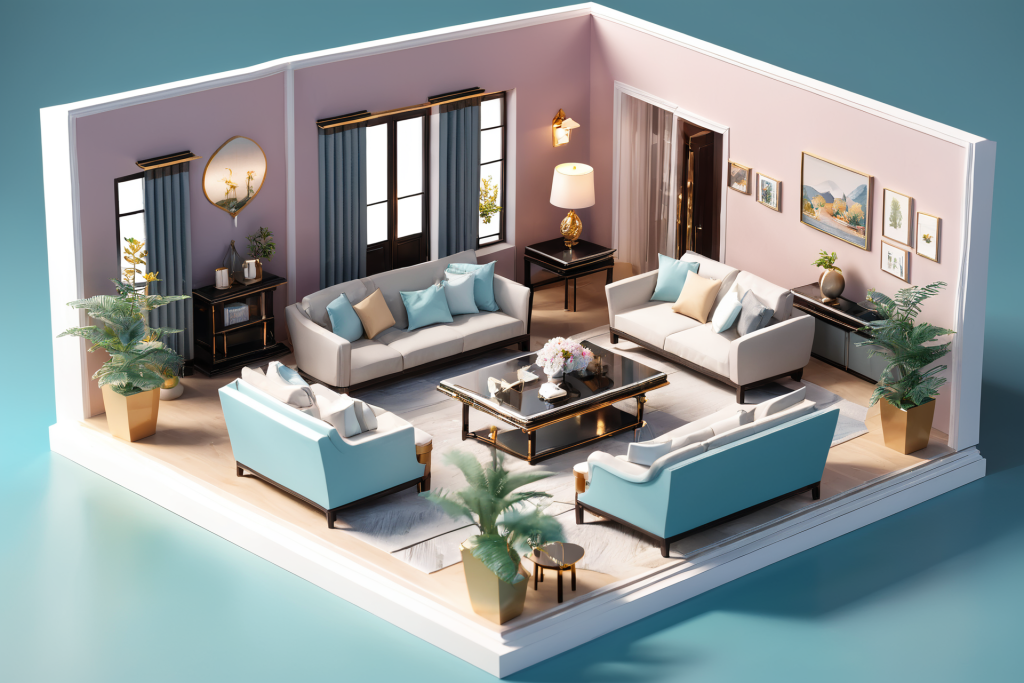
\includegraphics[width=0.4\textwidth]{graphic.png} %插入图形 graphic.png,缩放系数 scale=0.3。
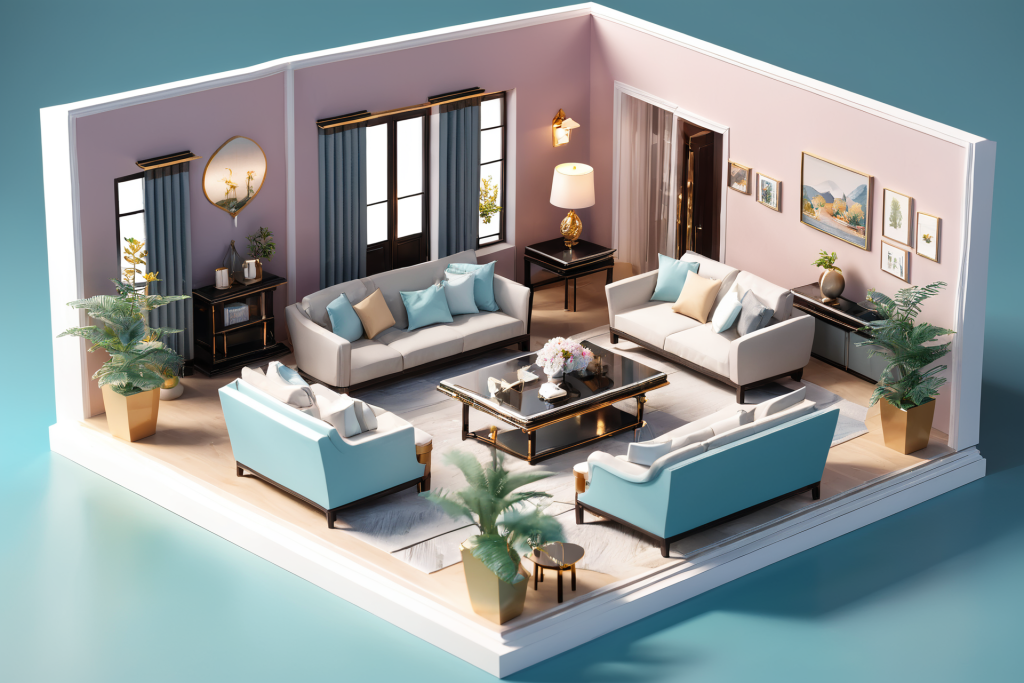
\includegraphics[angle=90,totalheight=40mm]{graphic.png}
%第 2 次插入图形 graphic.png,逆时针转 90 度,总高度为 40mm。
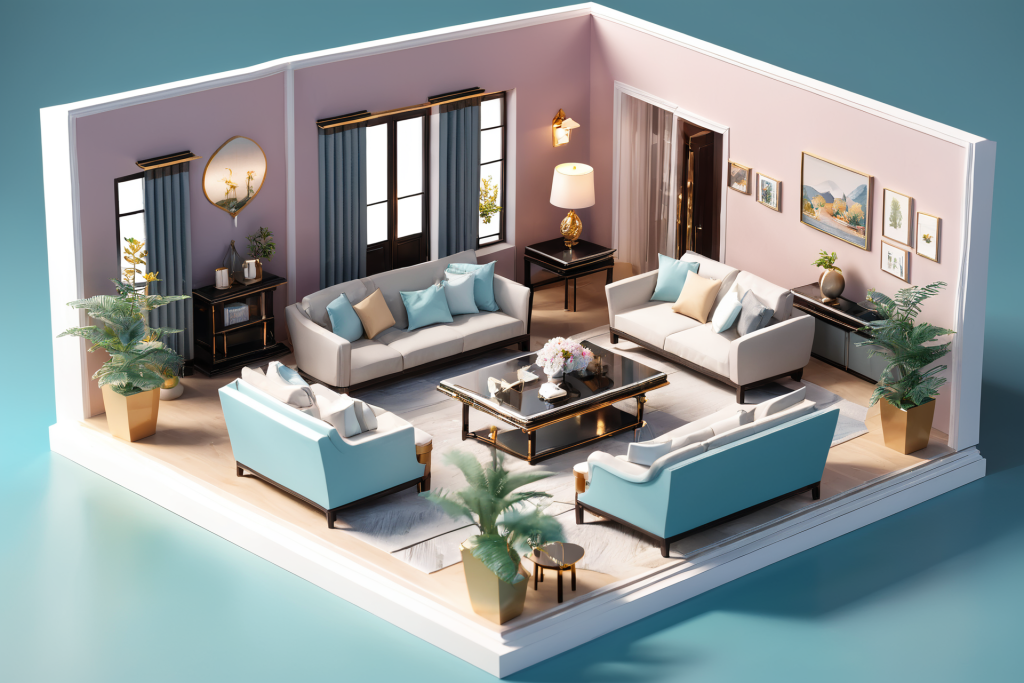
\includegraphics[totalheight=40mm,angle=270]{graphic.png}
%第 3 次插入图形 graphic.png,逆时针旋转 90 度,总高度为 40mm。
\end{figure} %结束浮动图形  环境。
\end{document} %结束文档。